\section{Tests results}
\label{performance_evaluation:tests_result}


\subsection{Rectangle test evaluation}
\label{performance_evaluation:tests_result:rectangletest}

Figure \subref{fig:rectangletest} shows the first test trajectory:
it is a rectangle. This path has been chosen for testing since it
features long straight segments and hard turnings (more than 80
degrees).

\begin{figure}[!htp]
  \begin{center}
    \subfigure[Rectangle trajectory test]{
      \label{fig:rectangletest}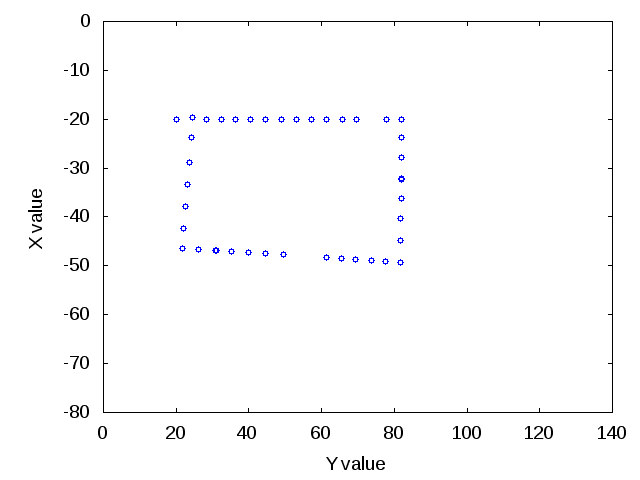
\includegraphics[width=300pt]{img/path_session_9.png}
    }

    \vspace*{30pt}
    \subfigure[Users' disturbance during the rectangle test by
      sudden change of the point-of-view over a 0/4 scale]{
      \label{fig:rectangledata}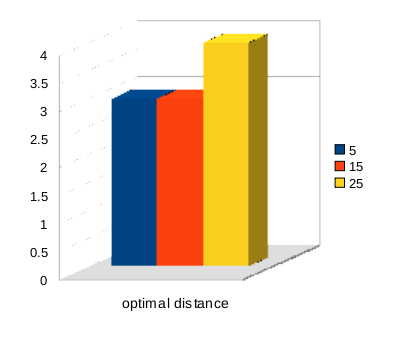
\includegraphics[width=200pt]{img/square.png}
    }
  \end{center}
  \caption{Rectangle test}
  \label{fig:rectangle}
\end{figure}

The result evidence is that most of the users figured out the
trajectory performed by the robot, even tough they perceived
sudden point of view changes during hard turnings.
\\
To sum up, they evaluated the experience positively when the
optimal distance were set to 5 or 25; not too comfortable
when set to 15.


\subsection{Ellipse test evaluation}
\label{performance_evaluation:tests_result:ellipsetest}

Figure \subref{fig:ellipsetest} shows the second test trajectory:
it is an ellipse. This path has been chosen for testing since it
features long smooth turns.

\begin{figure}[!htp]
  \begin{center}
    \subfigure[Ellipse trajectory test]{
      \label{fig:ellipsetest}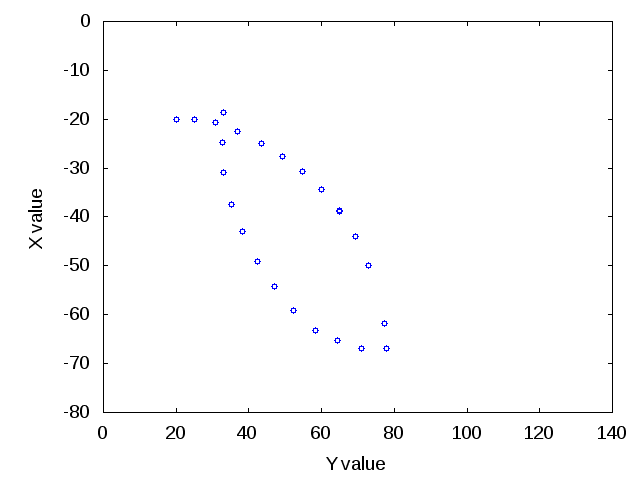
\includegraphics[width=300pt]{img/path_session_5.png}
    }

    \vspace*{30pt}
    \subfigure[Users' disturbance during the ellipse test by
      sudden change of the point-of-view over a 0/4 scale]{
      \label{fig:ellipsedata}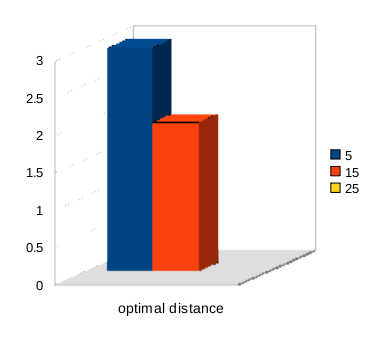
\includegraphics[width=200pt]{img/ellipse.png}
    }
  \end{center}
  \caption{Ellipse test}
  \label{fig:ellipse}
\end{figure}

The result evidence is that all of the users figured out the
trajectory performed by the robot. This case allows to point out
a specify trend: the more the optimal distance is, the less users
perceive sudden point of view changes.
\\
Testers also reported they had very comfortable experience.


\subsection{Broken lines test evaluation}
\label{performance_evaluation:tests_result:zigzagtest}

Figure \subref{fig:zigzagtest} shows the third test trajectory:
it is made up of broken lines. This path has been chosen for testing
since it features straight lines and sudden hard turnings.

\begin{figure}[!htp]
  \begin{center}
    \subfigure[Broken lines trajectory test]{
      \label{fig:zigzagtest}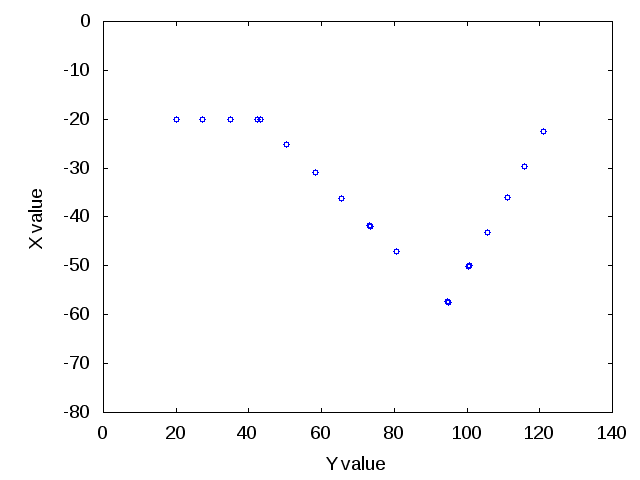
\includegraphics[width=300pt]{img/path_session_6.png}
    }

    \vspace*{30pt}
    \subfigure[Users' disturbance during the broken lines test by
      sudden change of the point-of-view over a 0/4 scale]{
      \label{fig:zigzagdata}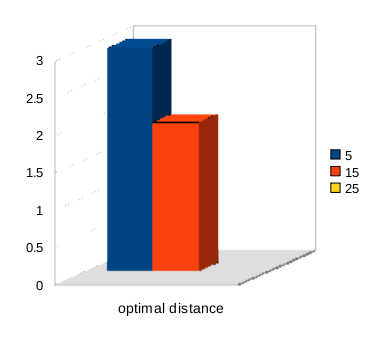
\includegraphics[width=200pt]{img/ellipse.png}
    }
  \end{center}
  \caption{Broken line test}
  \label{fig:zigzag}
\end{figure}

The result evidence is the users did not recognise the performed path.
Moreover, it also emerged that the more the optimal distance is short,
the less are the occurrences of sudden point of view changes.
\\
For the reasons above, testers reported a not very comfortable experience.
